% 20190401 V0.99 
% USE XELATEX: Tools->Befehle->XELATEX cause of font -> F2

\documentclass[12pt]{scrreprt}

\usepackage{amsmath}    % need for subequations
\usepackage{graphicx}   % need for figures
\usepackage{verbatim}   % useful for program listings
\usepackage{color}      % use if color is used in text
\usepackage{subfigure}  % use for side-by-side figures
\usepackage{hyperref}   % use for hypertext links, including those to external documents and URLs
\usepackage[german]{babel}
%\usepackage[utf8]{inputenc}
\usepackage{fancyhdr}
\usepackage{fontspec}
\setmainfont{Palatino Linotype}
\setsansfont{Palatino Linotype}
%\setmonofont{Palatino Linotype}

\usepackage[
headheight=62pt,
%textheight=600pt,
textwidth=470pt,
%footskip=30pt,
paperwidth=597pt,
footskip=40pt,
bottom=80pt,
% other options
]{geometry}


%Definieren uns farbigen Quellcode
\usepackage{color}
\definecolor{dkgreen}{rgb}{0,0.6,0}
\definecolor{gray}{rgb}{0.5,0.5,0.5}
\definecolor{mauve}{rgb}{0.58,0,0.82}

%Damit wir Quellcode nutzen können.
\usepackage{listings}
\lstset{numbers=left,
	numberstyle=\scriptsize,
	numbersep=8pt,
	breaklines=true,
	showstringspaces=false,
	frame=0,
	xleftmargin=15pt,
	xrightmargin=5pt,
	basicstyle=\ttfamily\small,
	stepnumber=1,
	keywordstyle=\color{blue},          % keyword style
	commentstyle=\color{dkgreen},       % comment style
	stringstyle=\color{mauve}         % string literal style
}


%Sprache Festelegen
\lstset{language=Matlab}

\pagestyle{fancy}

\fancyhf{}
\rhead{\includegraphics[height=1.5cm]{img/HAW_logo_black.png}}
\chead{P1 - Signale und Systeme 1}
\lhead{F. Lanz, M. Müller}

\cfoot{\thepage \, / 9}
\renewcommand{\footrulewidth}{0.4pt}
\renewcommand{\headrulewidth}{0.4pt}



\begin{document}

\begin{titlepage}
	
	
	\centering
	\begin{figure}
		\vspace*{1cm}	
	\end{figure}
	
	
	{\huge\bfseries P1 Frequenzgang und Fourier-Reihe\par}
	
	\vspace{1cm}
	
	{\LARGE Praktikum Signale und Systeme 1\par}
	
	\vspace{1.5cm}
	
	\includegraphics[width=7cm]{img/HAW_logo_black.png}\par
	\vspace{1.5cm}
	
	
	{\large \bfseries Finn Lanz \hspace{0.8cm} Malte Müller\par}
	
	\vspace{1.5cm}

	{\large \today\par}

	\vspace{3cm}

	\begin{tabular}{lr}
		\rule[-1ex]{0pt}{2.5ex} \textbf{Name} \hspace{2cm} & \textbf{Funktion }\\ 
		\rule[-1ex]{0pt}{2.5ex} Malte Müller & Protokollführer \\ 
		\rule[-1ex]{0pt}{2.5ex} Finn Lanz & Teilnehmer \\ 	
	\end{tabular} 

	\vfill
	{SS1P/2 - E-B3 - VLM} 
	\vspace{2cm}
	

		
	
\end{titlepage}

\tableofcontents
\thispagestyle{fancy}


\chapter{Vorbereitung}
\thispagestyle{fancy}

%Vorbereitung
\begin{center}
	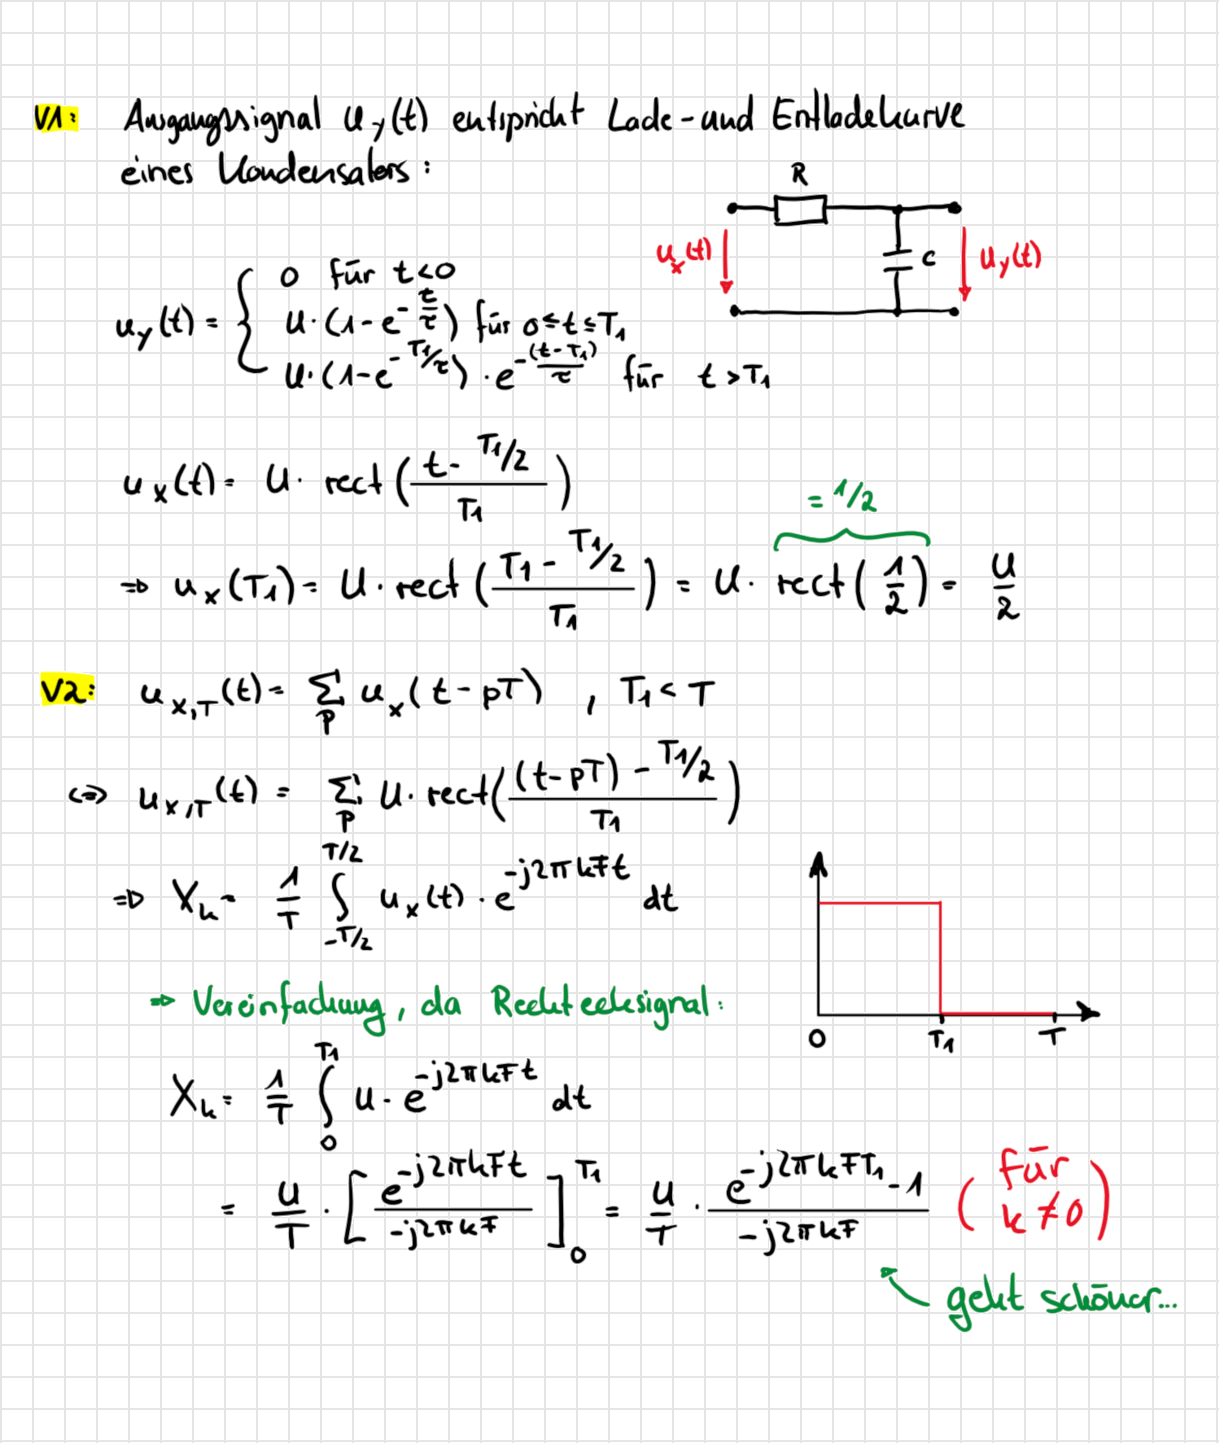
\includegraphics[]{img/ssp1_vorb1.png}
	\newpage
	\thispagestyle{fancy}
	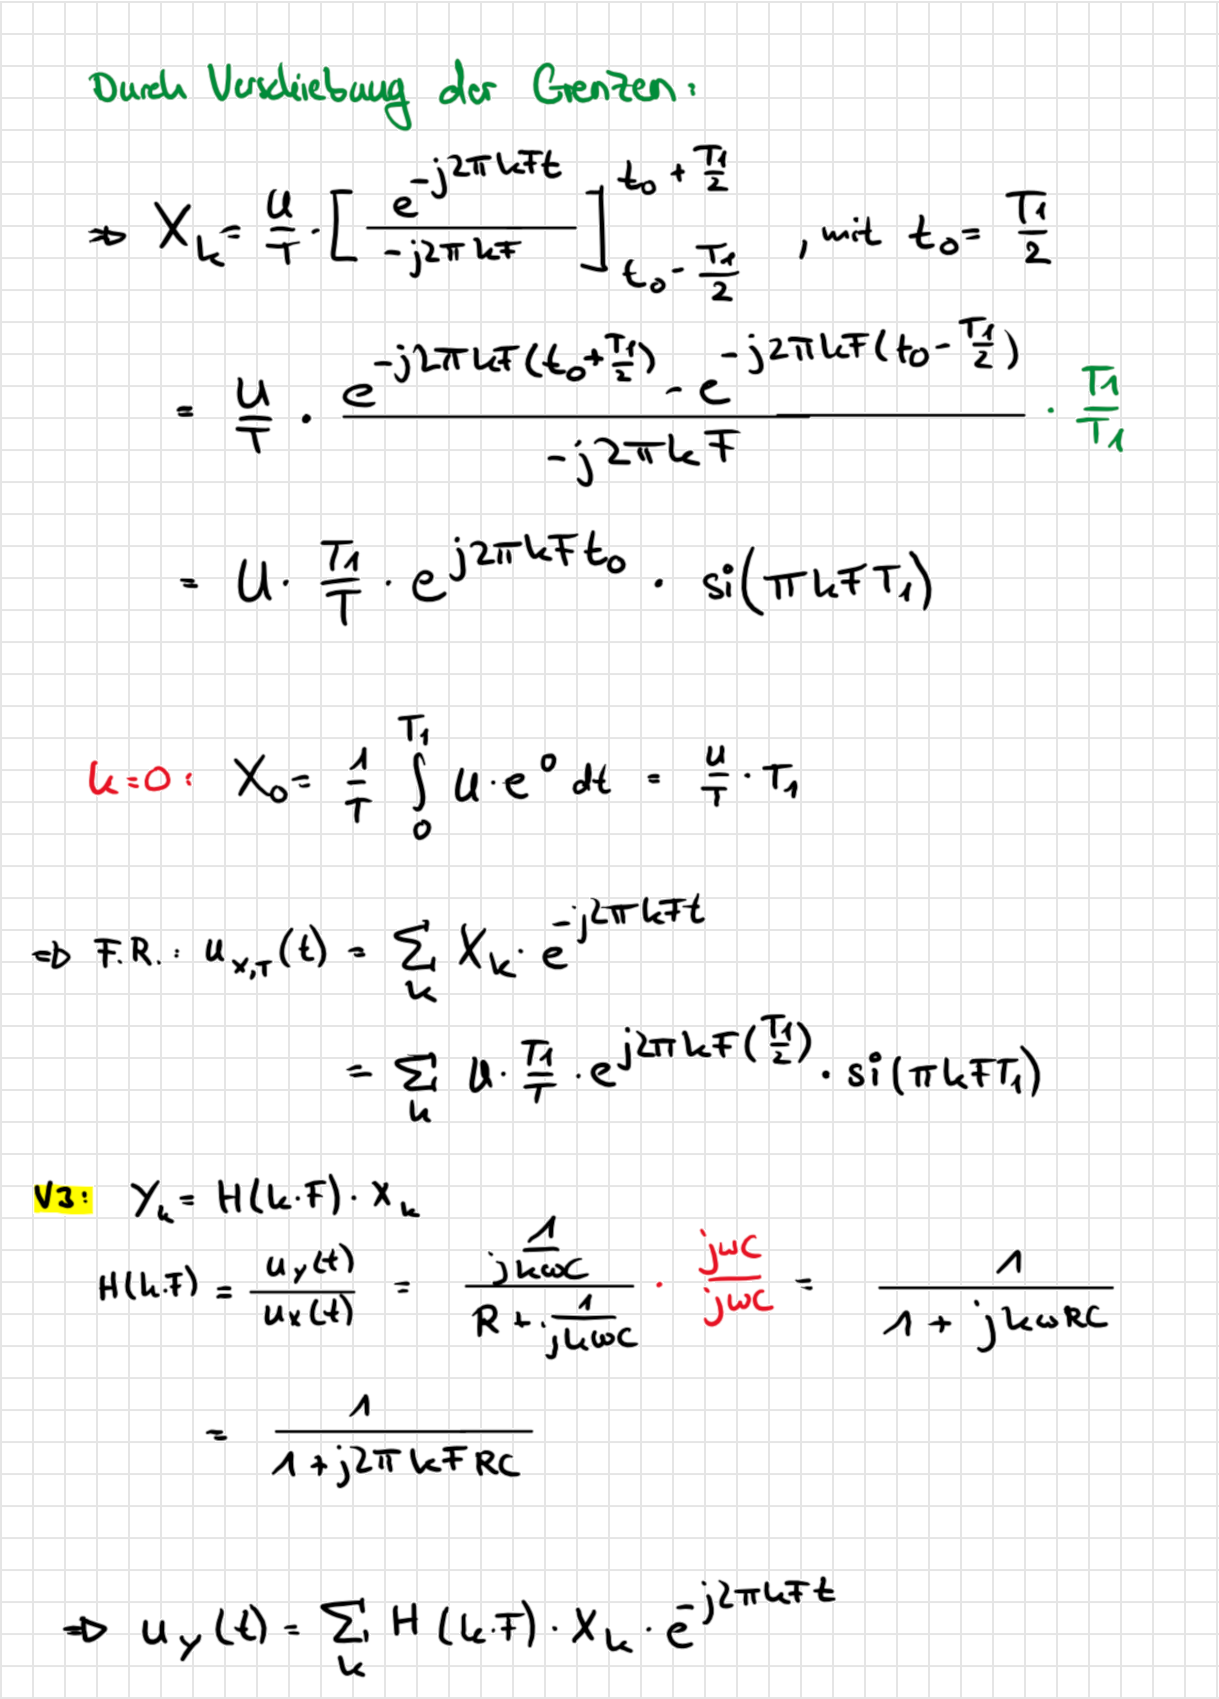
\includegraphics[]{img/ssp1_vorb2.png}
	\newpage
	\thispagestyle{fancy}
	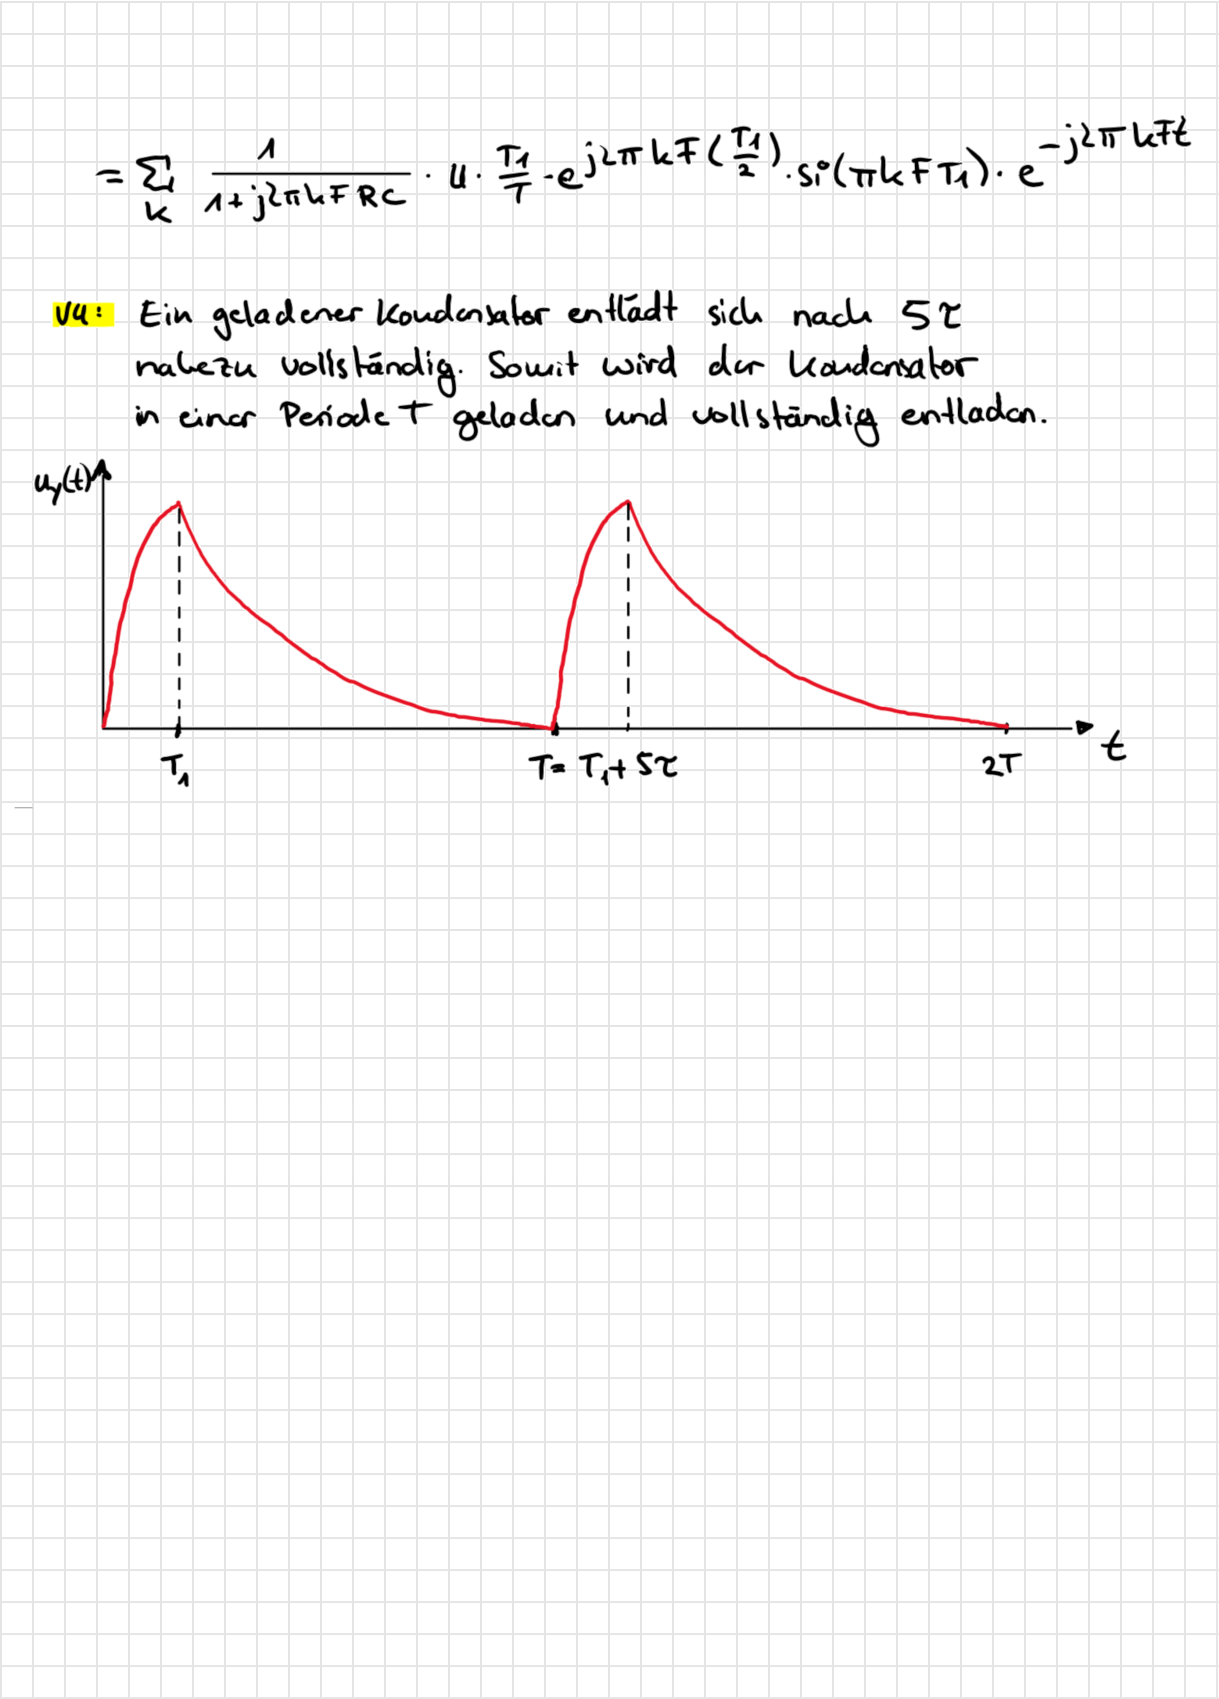
\includegraphics[]{img/ssp1_vorb3.png}
\end{center}

\chapter{Aufgaben im Labor}
\thispagestyle{fancy}

\section{Theoretische Lösung aus V1}

Die theoretische Ausgangsfunktion $u_y(t)$ soll mit Matlab programmiert und in einem Grafen dargestellt werden. 

\vspace{0.5cm}

\begin{lstlisting}
%% Aufgabe 1

% Berechnung der Lade- und Entladekurve

t1 = 0:dt:tau;              % Ladezeit
uy1 = U * (1-exp(-t1/tau)); % Ladefunktion

t2 = tau:dt:(tau+5*tau);    % Entladezeit
uy2 = U * (1-exp(-tau/tau)) * exp(-(t2-tau)/tau); % Entladefkt

uy = [uy1, uy2];    % Zusammensetzen der Lade- und Entladewerte
t = [t1, t2];

plot(t, uy); grid on; grid minor; %axis tight; 

% Beschriftung des Graphen:

title('Ausgangsspannung u_y(t)');
xlabel('t');
ylabel('u_y(t)');

\end{lstlisting}

\vspace{0.5cm}
    
Ausgegeben wird folgende Grafik:
\begin{center}
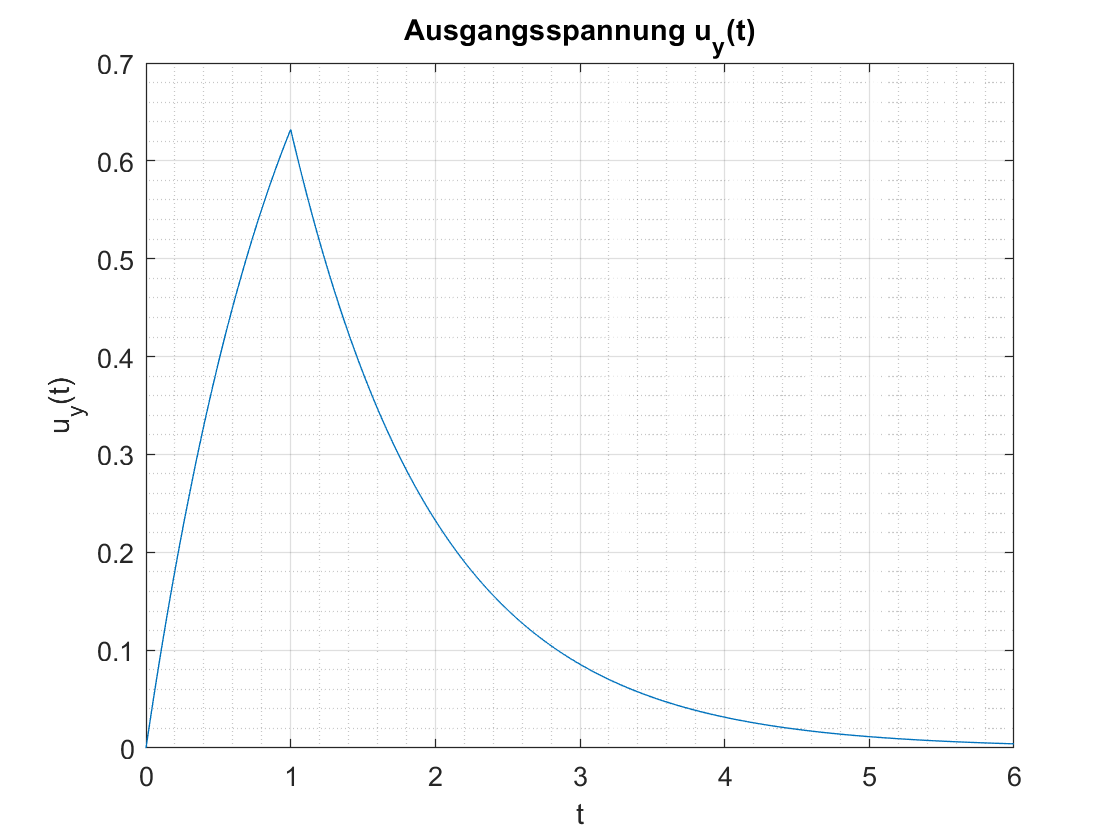
\includegraphics[width=200pt]{img/aufgabe1.png}
\end{center}


% include sections like this


\end{document}
